\documentclass{scrartcl}
\usepackage{amsmath}
\usepackage{graphicx}
\usepackage{url}
\usepackage{listings}
\renewcommand{\lstlistingname}{Listing}
\title{Linear Least Squares}
\subtitle{Version 1.0}
\author{R. Steven Turley}
\date{August 31, 2018}
\begin{document}
\maketitle
\tableofcontents

\section{Introduction}
This article describes how to find the best fit to a function
of the form
\begin{equation}
f(x;\vec{b})=\sum_{k=1}^{p} b_k g_k(x)\label{eq:lin}
\end{equation}
to a set of data points $(x_i,y_i)$.
It is linear in the sense that $f$ is linear in the parameters
$b_k$. It is called "least squares" because by "best fit" I
mean the function which finds the set
of parameters $b_k$ which minimizes $\chi^2$, the sum of the squares of
the differences between $f(x_i;\vec{b})$ and $y_i$.
\begin{equation}
\chi^2 = \sum_{i=1}^n [f(x_i;\vec{b})-y_i)]^2\label{eq:uwchi}
\end{equation}
If the data is heteroscedactic (i.e. if the extent of the deviations
of $y_i$ from $f(x_i,\vec{b})$ varies across the range of $x_i$, 
the appropriate function to minimize is a weighted sum of the squares.
This can be written in terms of the weights $w_i$ or in terms of the
relative uncertainties at each data point $\sigma_i$.
\begin{align}
\chi^2 &= \sum_i w_i[f(x_i;\vec{b})-y_i)]^2\label{eq:wchi}\\
\chi^2 &= \sum_i \left[\frac{f(x_i;\vec{b})-y_i)}{\sigma_i}\right]^2
	\label{eq:schi}\\
w_i &= \sigma_i^{-2}\label{eq:ws}
\end{align}

A good, but somewhat dated reference for the derivations here
is the current version of Bevington\cite{Bevington},
the book I first learned statics from. Some other helpful references
which helped me with these derivations are the article
in Wikipedia\cite{Wikipedia} and the article in
MathWorld\cite{MathWorld}.

A special case of linear least squares fitting in polynomial fitting
which will be considered separately in another article\cite{polyfit}.

\section{Finding Parameters}
The function $\chi^2$ can be minimized by finding the point
where it's gradient is zero.
%\begin{equation}
%\nabla_\vec{b} \chi^2
%\end{equation}
This is true if all of the partial derivatives\footnote{A
partial derivative $\partial/b_i$ is the derivative with respect
to $b_i$ holding all other quantities constant.}
of $\chi^2$ with
respect to the parameters $b_i$ are equal to zero. In the case 
of unweighted least squares in Eq.~\ref{eq:uwchi}
\begin{align}
\frac{\partial \chi^2}{\partial b_j} &= \frac{\partial}{\partial b_j}
\sum_i [f(x_i;\vec{b})-y_i)]^2\\
	&= 2\sum_i [f(x_i;\vec{b})-y_i)]
		\left(\frac{\partial f(x_i;\vec{b})}{\partial b_j}\right).
		\label{eq:lpart}\\
	&= 0
\end{align}
The partial derivative is simple when $f$ has the linear form
in Eq.~\ref{eq:lin}.
\begin{equation}
\partial{f(x;\vec{b})}{\partial b_j} = g_j(x)\label{eq:linpart}
\end{equation}
Substituting Eq.~\ref{eq:lin} and Eq.~\ref{eq:linpart} into
Eq.~\ref{eq:lpart},
\begin{align}
0 &= \sum_i [f(x_i;\vec{b})-y_i)]g_j(x_i)\\
	&= \sum_i \left[\sum_k b_k g_k(x_i)-y_i\right]g_j(x_i)\\
	\sum_{i,k} g_k(x_i)g_j(x_i)b_k.&= \sum_i g_j(x_i)y_i.\label{eq:linsolve}
\end{align}
If there are $p$ parameters $b_k$, Eq.~\ref{eq:linsolve} represents
$p$ linear equations with $p$ unknowns which can be written in
matrix form.
\begin{equation}
\left(\begin{array}{ccc}
\sum_i g_1(x_i)^2&\cdots&\sum_i g_1(x_i)g_p(x_i)\\
\vdots&\vdots&\vdots\\
\sum_i g_n(x_i)g_1(x_i)&\cdots&\sum_i g_n(x_i)g_p(x_i)
\end{array}\right)
\left(\begin{array}{c}
b_1\\
\vdots\\
b_p
\end{array}\right) =
\left(\begin{array}{c}
\sum_i g_1(x_i)y_i\\
\vdots\\
\sum_i g_p(x_i)y_i
\end{array}\right)\label{eq:uwmat}
\end{equation}
Eq.~\ref{eq:uwmat} can be solved for the parameters $b_k$
using standard matrix techniques.

The weighted fits in Eq.~\ref{eq:wchi} can similar be solved.
\begin{equation}
\left(\begin{array}{ccc}
\sum_i w_i g_1(x_i)^2&\cdots&\sum_i w_i g_1(x_i)g_p(x_i)\\
\vdots&\vdots&\vdots\\
\sum_i w_i g_n(x_i)g_1(x_i)&\cdots&\sum_i w_i g_n(x_i)g_p(x_i)
\end{array}\right)
\left(\begin{array}{c}
b_1\\
\vdots\\
b_p
\end{array}\right) =
\left(\begin{array}{c}
\sum_i w_i g_1(x_i)y_i\\
\vdots\\
\sum_i w_i g_p(x_i)y_i
\end{array}\right)\label{eq:wmat}
\end{equation}
Substituting Eq.~\ref{eq:ws} into Eq.~\ref{eq:wmat}
gives the equation for weighted linear least squares
in terms of the uncertainties $\sigma_i$.
\begin{multline}
\left(\begin{array}{ccc}
\sum_i g_1(x_i)^2/\sigma_i^2&\cdots&\sum_i g_1(x_i)g_p(x_i)/\sigma_i^2\\
\vdots&\vdots&\vdots\\
\sum_i g_n(x_i)g_1(x_i)/\sigma_i^2&\cdots&\sum_i g_n(x_i)g_p(x_i)/\sigma_i^2
\end{array}\right)
\left(\begin{array}{c}
b_1\\
\vdots\\
b_p
\end{array}\right) =\\
\left(\begin{array}{c}
\sum_i g_1(x_i)y_i/\sigma_i^2\\
\vdots\\
\sum_i g_p(x_i)y_i/\sigma_i^2
\end{array}\right)\label{eq:smat}
\end{multline}
If the $g_k$ are monomials with $g_k(x_i)=x_i^{k-1}$, then
Eq.~\ref{eq:uwmat} takes on a particularly simple form.
\begin{equation}
\left(\begin{array}{ccc}
n&\cdots&\sum_i x_i^{p-1}\\
\vdots&\vdots&\vdots\\
\sum_i x_i^{n-1}&\cdots&\sum_i x_i^{n+p-2}
\end{array}\right)
\left(\begin{array}{c}
b_1\\
\vdots\\
b_p
\end{array}\right) =
\left(\begin{array}{c}
\sum_i y_i\\
\vdots\\
\sum_i x_i^{p-1}y_i
\end{array}\right)
\end{equation}
Fitting polynomials is discussed further in my polynomial fitting
article\cite{polyfit}.

\section{Residuals}
A measure of the quality of the fit are the residuals $r_i$, which
are the differences between the data points $y_i$ and the
fit function $f$.
\begin{equation}
r_i = y_i - f(x_i;\vec{b})
\end{equation}
It is always a good idea to plot the residual or the fit
and the data when you're fitting
to make sure it looks reasonable. Two common problems which
are easy to spot graphically are an inaccurate or incomplete
set of functions $g_k$ and incorrect weights $w_i$.
Fig.~\ref{fig:quaddata} is some data from a quadratic function
with noise.
\begin{figure}
\begin{center}
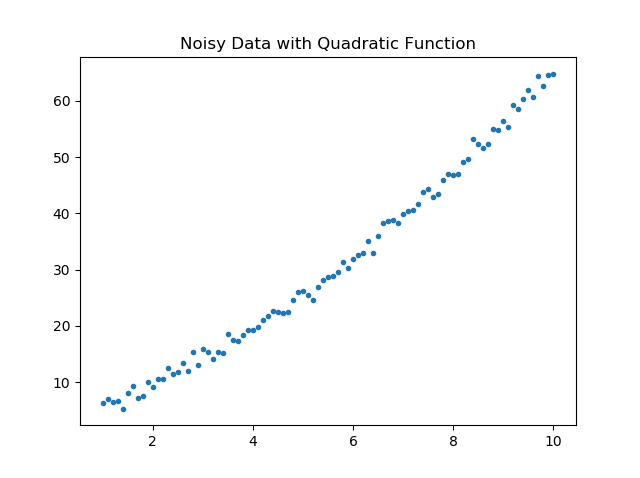
\includegraphics[width=11cm]{quaddata}
\end{center}
\caption{\label{fig:quaddata}Quadratic function with random
noise added.}
\end{figure}
I fit the data with a linear function $y=mx+b$ and plotted the
residual in Fig.~\ref{fig:lin2quad}.
\begin{figure}
\begin{center}
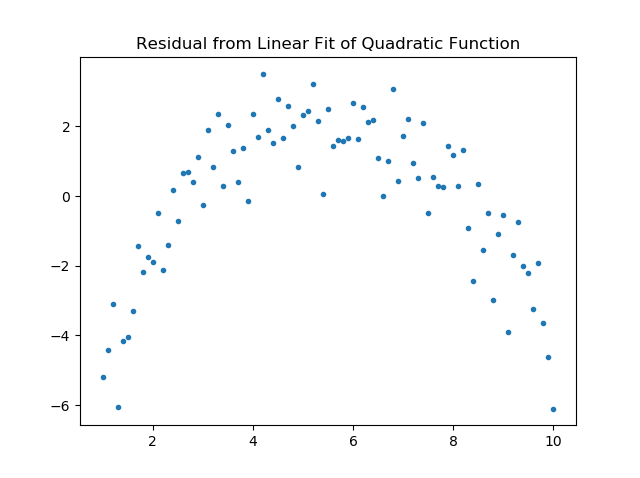
\includegraphics[width=11cm]{lin2quad}
\end{center}
\caption{\label{fig:lin2quad}Residual from the fit of the
data in Fig.~\ref{fig:quaddata} to a straight line.}
\end{figure}
Notice how the residual jumps around but is characteristically below
zero for parts of the and characteristically above zero for other
parts. This is characteristic of using a wrong or incomplete function
top fit the data. If I fit the data to a quadratic curve,
I get the residual in Fig.~\ref{fig:quadfit}.
\begin{figure}
\begin{center}
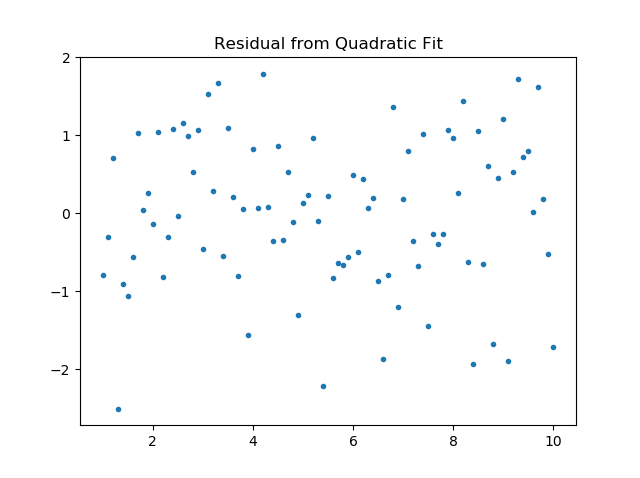
\includegraphics[width=11cm]{quadfit}
\end{center}
\caption{\label{fig:quadfit}Residual from the fit of the
data in Fig.~\ref{fig:quaddata} to a quadratic polynomial.}
\end{figure}
Notice how the data is randomly on either side of the origin
in this case.

The need for a weighted fit can be illustrated by fitting the
data in Fig.~\ref{fig:epropy}.
\begin{figure}
\begin{center}
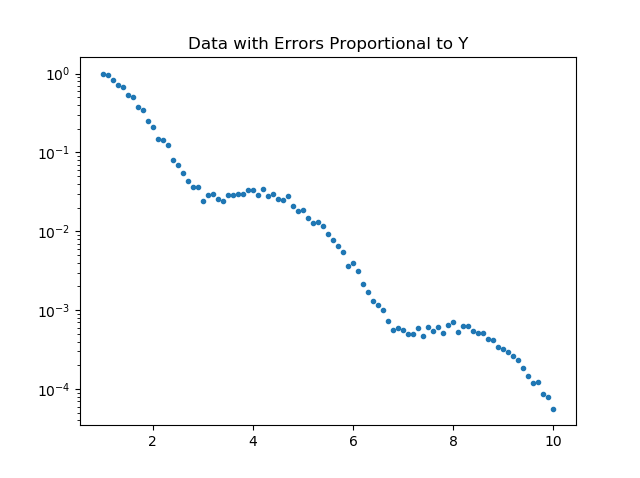
\includegraphics[width=11cm]{epropy}
\end{center}
\caption{\label{fig:epropy}Data with large differences
in magnitude and an error which is proportional to the
signal.}
\end{figure}
Fig.~\ref{fig:dfeq} shows the data and the fit when I use
equal weights at each point (i.e. an unweighted fit). Notice
that the fit is considerable closer to the data points in the
region where the function is large compared to the region
where the function is small.
\begin{figure}
\begin{center}
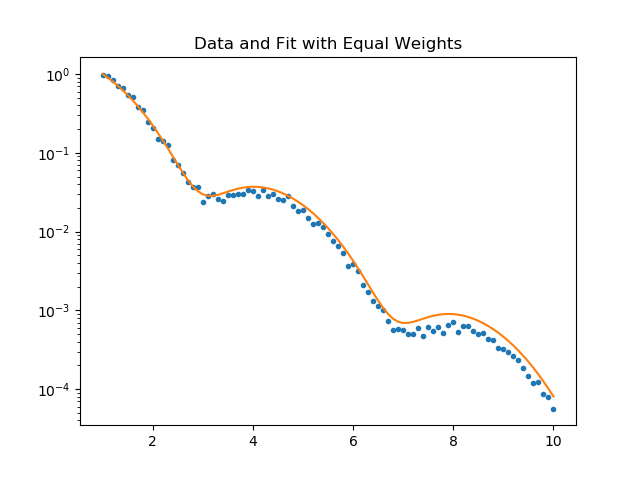
\includegraphics[width=11cm]{dfeq}
\end{center}
\caption{\label{fig:dfeq}Data and fit for the data
in Fig.~\ref{fig:epropy} using equal weights.}
\end{figure}
Fig.~\ref{fig:dfpw} is a fit to the same data using the same
fit function but with weights proportional to the signal.
\begin{figure}
\begin{center}
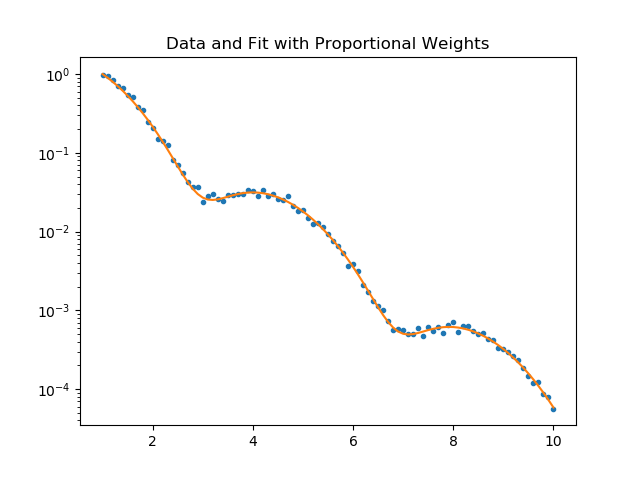
\includegraphics[width=11cm]{dfpw}
\end{center}
\caption{\label{fig:dfpw}Data and fit for the data
in Fig.~\ref{fig:epropy} using proportional weights.}
\end{figure}

\section{Parameter Uncertainties}\label{sec:uncert}
As shown in my general uncertainties article\cite{uncertainties},
the uncertainties in the fit parameters can be estimated from
covariance matrix $C$ which can be computed from the Jacobian
$J$.
\begin{equation}
J = \left(\begin{array}{ccc}
\partial f(x_1;\vec{b})/\partial b_1& \cdots &
	\partial f(x_1;\vec{b})/\partial b_p\\
\vdots & \vdots & \vdots \\
\partial f(x_n; \vec{b})/\partial b_1 & \cdots  &
	\partial f(x_n;\vec{b})/\partial b_p
\end{array}\right).
\end{equation}
From Eq.~\ref{eq:lin}, it is apparent that
\begin{equation}
\frac{\partial f(x_i;\vec{b})}{\partial b_k} = g_k(x_i)
\end{equation}
so that
\begin{equation}
J = \left(\begin{array}{ccccc}
g_1(x_1)&g_2(x_1)& \cdots & g_{p-1}(x_1)& g_p(x_1)\\
g_1(x_2)&g_2(x_2)& \cdots & g_{p-1}(x_2)& g_p(x_2)\\
\vdots & \vdots & \vdots & \vdots & \vdots\\
g_1(x_{n-1}) & g_2(x_{n-1}) & \cdots & g_{p-1}(x_{n-1}) & g_p(x_{n-1})\\
g_1(x_n) & g_2(x_nj) & \cdots & g_{p-1}(x_n) & g_p(x_n)
\end{array}\right).
\end{equation}
The covariance matrix $C$ can be computed from $J$.
\begin{equation}
C = s_y^2(J^{T}J)^-1
\end{equation}
The uncertainty in $y$, $s_y$ can be estimated from the residuals
\begin{equation}
r_i = y-i - f(x_i;\vec{b})
\end{equation}
where $\vec{b}$ has the best values from the fit.
\begin{equation}
s_y \approx \frac{1}{n-p}\sum r_i^2.
\end{equation}
The uncertainty in the fit parameter $b_i$ is
\begin{equation}
s_i = \sqrt{C_{ii}}\;.
\end{equation}

\appendix

\section{Computer Codes}

\subsection{Excel}\label{sec:excel}
The original motivation for this work was to understand
the output of a regression analysis in Excel. After installing
the Data Analysis Add-in, I saw the following section
in the Data tab.
\begin{center}
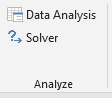
\includegraphics{analbox}
\end{center}
I clicked on the Data Analysis item and it brought up the following
menu.
\begin{center}
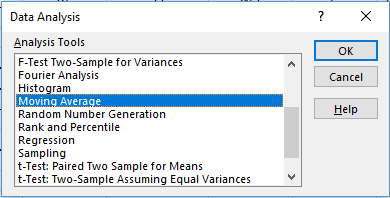
\includegraphics{analmenu}
\end{center}
I picked the Random Number Generation item to create a normally
distributed 5 random numbers in Column~A with mean 0 and standard
deviation 1.

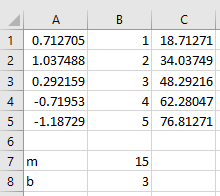
\includegraphics{ABC}

I filled column B with the x values I wanted to fit and set
column C using the following formula for example for
cell C2: \texttt{=A2+$B$7*B2+$B$8}.
Then I went back to the Data Analysis menu and selection regression.
The y input range was the data in Column C. The x input range was
the data in column B. The output range was the cell E1. The
data I was most interested in from the regression was the
second table under the ANOVA heading.

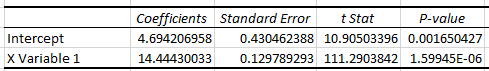
\includegraphics{anova1}

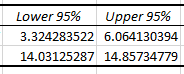
\includegraphics{anova2}

This is the data I wanted to understand by comparing it with the
output of other programs. I determined that the coefficients were
what one gets doing a linear least squares fit as outlined
in this article. It agreed with the other programs I tried.
Likewise, the Standard Error column is the estimated standard
deviation in the fit parameters as computed by other programs.
The t-stat column is the ratio of the coefficient to the
standard deviation. The P-value is (correctly calculated
as following from the integral of the Student t distribution
$s(t,\nu)$ where $t$ is the t statistic described earlier and
$\nu$ is the number of degrees of freedom. It is equal to 3 in
this case, the
number of data points (5) minus the number of
fit parameters (2).
\begin{equation}
p=2*\left(1-\int_{\tau=0}^t s(\tau,\nu)\right)
\end{equation}
\subsection{MATLAB}
I duplicated the Excel calculation in Matlab using the
polyfit routine and their prescription for calculating
the standard errors using the information in the S structure.
\begin{lstlisting}
% Polynomial fit coefficient uncertainties
noise=[0.712705059,
1.037487891,
0.292159257,
-0.71952627,
-1.187286216]';
m=15;
b=3;
x=1:5;
y=noise + m*x + b;
[p,S] = polyfit(x,y,1);
p
ste = sqrt(diag(inv(S.R)*inv(S.R')).*S.normr.^2./S.df)
\end{lstlisting}
You'ree note that these values agree with the Excel calculations.

\subsection{Mathematica}
Here is the Mathematica code I used to reproduce the Excel
calculation.
\begin{lstlisting}
noise = {0.712705059,
  1.037487891,
  0.292159257,
  -0.71952627,
  -1.187286216};
x = Range[1, 5];
m = 15.;
b = 3.;
y = noise + m*x + b
data = Transpose[{x, y}];
lm = LinearModelFit[data, w, w];
lm["ParameterTable"]
\end{lstlisting}
It produced the following output, which agreed with Excel.

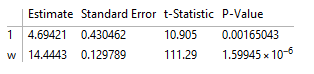
\includegraphics{mathout}

I also did a distribution check to see if average estimated
variance in the fit parameters matched the actual variance 
in those parameters with 10,000 different random noise
samples. Here is the Module to compute the fit parameters
and parameter error estimates.
\begin{lstlisting}
myFit[] := Module[{noise, m = 15., b = 3., x, y, data, lm, w},
  x = Range[1, 5];
  noise = RandomReal[NormalDistribution[], 5];
  y = noise + m*x + b;
  data = Transpose[{x, y}];
  lm = LinearModelFit[data, w, w];
  Join[lm["BestFitParameters"], lm["ParameterErrors"]]]
\end{lstlisting}
Here is the code to do the 10,000 trials.
\begin{lstlisting}
trials = 10000;
pars = Table[myFit[], {i, trials}];
spars = Total[pars]/trials
ssqpars = Total[pars*pars]/trials;
Sqrt[ssqpars - spars^2]
\end{lstlisting}
The results were as follows.
\begin{lstlisting}
{2.98924, 15.003, 0.962881, 0.29032}
{1.05124, 0.314441, 0.408231, 0.123086}
\end{lstlisting}
These don't agree with each other as well as my Julia results
and I'm not sure why. However, they are close enough (within 10\%)
that I'm not too concerned.
\subsection{Python}
The following python code was intended to calculate the same thing
as in the other languages.
\begin{lstlisting}
# -*- coding: utf-8 -*-
"""
Created on Fri Aug 31 12:00:20 2018

@author: rstur_000
"""
import numpy as np
# import matplotlib.pyplot as plt

noise=[0.712705059,
    1.037487891,
    0.292159257,
    -0.71952627,
    -1.187286216]
m=15
b=3
x=np.linspace(1,5,5)
y=noise+m*x+b

p, cov = np.polyfit(x,y,1,full=False, cov=True)
pfit = np.poly1d(p)
yfit = pfit(x)
res = y-yfit
mse = sum(res*res)/3
sigma = np.sqrt(mse)
print("fit standard deviation in y = {:.4f}".format(sigma))
std = np.sqrt(np.diag(cov))
print("slope     = {:8.5f} +/- {:.5f}".format(p[0],std[0]))
print("intercept = {:8.5f} +/- {:.5f}".format(p[1],std[1]))
print("adjusted slope error is {:.4f}".format(std[0]/sigma))
print("adjusted intercept error is {:.4f}".format(
	std[1]/sigma))

# Try something else
p, cov = np.polyfit(x, y, 1, cov=True)

# Test these variances, they disagree with everyone else
sump = np.zeros(2)
sumsq = np.zeros(2)
sumstd = np.zeros(2)
trials=100
for i in range(100):
    noise = np.random.normal(size=5)
    y = noise + m*x + b
    p, cov = np.polyfit(x,y,1,full=False, cov=True)
    sump += p
    sumsq += p**2
    sig = np.sqrt(np.diag(cov))
    sumstd += sig
meanp = sump/trials
meansq = sumsq/trials
meanstd = sumstd/trials
calcstd = np.sqrt(meansq-meanp**2)
print("calculted std = {:.5f}, {:.5f}".format(calcstd[0],
	calcstd[1]))
print("mean std: ",meanstd)
print("meanstd/calcstd = ", meanstd/calcstd)
\end{lstlisting}
The output disagrees with the other programs. It gets the same
fit parameters, but different calculated uncertainties. The
distribution of fit parameters were similar to the other
programs.
\begin{lstlisting}
fit standard deviation in y = 0.4104
slope     = 14.44430 +/- 0.22480
intercept =  4.69421 +/- 0.74558
adjusted slope error is 0.5477
adjusted intercept error is 1.8166
calculted std = 0.29739, 1.04233
mean std:  [0.49968945 1.65728242]
meanstd/calcstd =  [1.68022641 1.58997506]
\end{lstlisting}

\subsection{Julia}
Most of the lengthy calculations and checks for the derivations
in this article were done with Julia. In the following section
I will list code snippets from the \texttt{LsqFit} module which
I used for the core of these calculations. That is followed
by a section with code used to produce the figures in this
report and test the results.
\subsubsection{LsqFit.jl}
I rewrote the library routine \texttt{LsqFit.jl}
to fix some problems in the routines and to work with
Julia 1.0. I also added some linear and polynomial curve
fitting routines and used the BFGS fitting routine
instead of the Levenberg-Marguardt routine it used (and which
I regard as inferior in most cases). This section has
snippets of the code form the LsqFit module and comments.

The module uses the CurveFitResult concrete type to store
the results of both linear and nonlinear fits.
\begin{lstlisting}
struct CurveFitResult
    dof::Int
    param::Vector{Float64}
    resid::Vector{Float64}
    jacobian::Matrix{Float64}
    converged::Bool
    wt::Array{Float64}
    mse::Float64
end
\end{lstlisting}
The \texttt{dof} variable is the number of degrees of freedom in the fit.
This is equal to the number of data points minus the number of
fit parameters.
The \texttt{param} vector are the fitted parameters. The \texttt{resid}
is the residual (the difference between the fit and the data at each
x point. The \texttt{jacobian} is the Jacobian of the fit function
which is explained in Sec.~\ref{sec:uncert}. For nonlinear fits,
\texttt{converged} is set equal to true if the fit converges. The
parameters are still updated, even if the fit doesn't converge and
may still be useful. The \texttt{wt} vector is the vector if
weights passed to the fitting function. If no weights are supplied,
this is set equal to a vector of ones. The \texttt{mse} field is
the mean square error. Is is the sum of the squares of the residuals
divided by the number of degrees of freedom.

The \texttt{curve\_fit} function fits data to a model
using a nonlinear least squares algorithm.
\begin{lstlisting}
function curve_fit(model::Function,
		xpts::AbstractArray, ypts::AbstractArray,
		wt::AbstractArray, p0::Vector; kwargs...)
    # construct a weighted cost function, with a vector weight
    # for each ydata. For example, this might be
    # wt = 1/sigma where sigma is some error term
    f(p) = wt .* ( model(xpts, p) - ypts )
    ssq(p) = sum(abs2, f(p))
    results = optimize(ssq, p0, BFGS(),
        Optim.Options(x_tol = 1e-10,
            f_tol = 1e-10,
            iterations = 10_000))
    # Fill the result with useful data
    dof = length(xpts) - length(p0)
    p = Optim.minimizer(results)
    res = f(p)
    g = Calculus.jacobian(f)
    jac = g(p)
    conv = Optim.converged(results)
    mse = sum(abs2, res)/dof
    CurveFitResult(dof, p, res, jac, conv, wt, mse)
end
\end{lstlisting}
The routine takes five required arguments and permits (but ignores)
optional arguments.
\begin{description}
\item{model:} a function with two parameters x and p
that computes the fit function with a given set of parameters
at the vector of data $x$.
\item{xpts:} the $x_i$ data points
\item{ypts:} the $y_i$ data points
\item{wt:} an array of weights used to weight the residual.
Note that it uses the weight differently than described in this
article. The variable $w_i$ in Eq.\ref{eq:wchi} is the square
of the elements in the passed \texttt{wt} array.
\item{p0:} the initial guess for the parameter values. Since
nonlinear least squares is an iterative technique, it needs
a starting point.
\end{description}
The routine defines the function \texttt{f(p)} to be the 
weighted residual at each step between the model and the data.
The \texttt{ssq} function is the sum of squares of the weighted
residuals and is what the optimizer minimizes. The routine
uses the \texttt{optimize} function from the library
\texttt{Optim} package to do the optimization. I've chosen to do
use the BFGS (Broyden-Fletcher-Goldfarb-Shanno) method, which
has worked well for me over the years. The options are set to
allow convergence under most normal conditions using numerical
derivatives in the gradient and hessian. After the fit is
complete, the numerical jacobian is calculated using the
\texttt{Calculus} package and the results are returned
as a \texttt{CurveFitResult} type.

The \texttt{linear\_fit} function does the unweighted
linear least squares calculations which are the focus of
this paper.
\begin{lstlisting}
function linear_fit(basis::AbstractArray, xpts::AbstractArray,
        ypts::AbstractArray)
    order=length(basis)
    A=zeros(order,order)
    y=zeros(order)
    for i=1:order
        for j=1:order
            A[i,j] = sum(basis[i](xpts).*basis[j](xpts))
        end
        y[i] = sum(ypts.*basis[i](xpts))
    end
    b = A\y
    npts = length(xpts)
    dof = npts-order
    yf = zeros(npts)
    for i=1:order
        yf += b[i].*basis[i](xpts)
    end
    res = yf .- ypts
    jac=Matrix{Union{Missing, Float64}}(missing,order,npts)
    for i=1:order
        jac[i,:] = basis[i](xpts)
    end
    conv = true
    wt = ones(npts)
    mse = sum(abs2, res)/dof
    CurveFitResult(dof, b, res, jac', conv, wt, mse)
end
\end{lstlisting}
It has three calling parameters.
\begin{description}
\item{basis:} an array of basis functions by which the
fit parameters are multiplied
\item{xpts}an array of the independent variables
\item{ypts}an array of the dependent variables to be fit
\end{description}
No initial guesses are required in this case since the fit
parameters \texttt{b} can be computed directly. The array
\texttt{yf} is the fit function evaluated with the final fit
parameters. As noted in Sec.~\ref{sec:uncert}, the Jacobian
can be computed directly in this case. Note that this routine
uses unweighted fitting and an unweighted Jacobian.

The \texttt{poly\_fit} function is a special case of the
\texttt{linear\_fit} function which it calls directly.
\begin{lstlisting}
function poly_fit(order::Int, xpts::AbstractArray,
		ypts::AbstractArray)
    lf = [x->x.^i for i=0:order]
    linear_fit(lf, xpts, ypts)
end
\end{lstlisting}
The only difference between these two functions if that the
\texttt{poly\_fit} function takes the order of the
polynomial to fit as its first argument. From that, it
computes the array of basis functions needed by
\texttt{linear\_fit}.

The \texttt{standard\_error} function estimates the uncertainties
in the fit parameters as explained in Sec.~\ref{sec:uncert}.
\begin{lstlisting}
function standard_error(fit::CurveFitResult;
		rtol::Real=NaN, atol::Real=0)
    # computes standard error of estimates from
    #   fit   : a CurveFitResult from a curve_fit()
    covar = estimate_covar(fit)
    # then the standard errors are given by the
    # sqrt of the diagonal
    vars = diag(covar)
    # Take the absolute value to be safe
    sqrt.(abs.(vars*fit.mse))
end
\end{lstlisting}
It uses the \texttt{estimate\_covar} routine to
estimate the covariance from the Jacobian and then
calculates the uncertainties from the diagonals of
the covariance matrix.
\begin{lstlisting}
function estimate_covar(fit::CurveFitResult)
    # computes covariance matrix of fit parameters
    J = fit.jacobian
    inv(J'*J)
end
\end{lstlisting}

\subsubsection{Code for Figures}
Here is the code I used to generate Fig.~\ref{fig:quaddata}.
\begin{lstlisting}
xpts = collect(1:0.1:10);
ypts = 2.0 .+ 3.0.*xpts .+ xpts.^2 ./3;
yn = ypts + randn(length(xpts));
import PyPlot
const plt = PyPlot;
plt.plot(xpts,yn,".")
plt.title("Noisy Data with Quadratic Function")
\end{lstlisting}
The two residual plots in Fig.~\ref{fig:lin2quad} and
Fig.~\ref{fig:quadfit} were generated with the following
code.
\begin{lstlisting}
cft = poly_fit(1, xpts, yn);
plt.plot(xpts,cft.resid,".");
plt.title("Residual from Linear Fit of Quadratic Function");
cft = poly_fit(2, xpts, yn);
plt.plot(xpts,cft.resid,".");
plt.title("Residual from Quadratic Fit")
\end{lstlisting}
Because I haven't implemented a weighted linear least squares
routine yet, I used the \texttt{curve\_fit} function for
Fig.\ref{fig:epropy}, Fig.~\ref{fig:dfeq}, and Fig.~\ref{fig:dfpw}.
\begin{lstlisting}
f(x,p)=exp.(-p[1].*(x.-1)) .*
	(0.8.*(cos.(p[2].*(x.-1))).^2 .+ 0.2)
ypts=f(xpts,p0);
yn = ypts.*(1 .+ randn(length(xpts))./10);
wt = 0.1.*ones(length(xpts))
cft = curve_fit(f, xpts, yn, wt, p0);
yft = f(xpts, cft.param);
plt.semilogy(xpts,yn,".",xpts,yft,"-")
plt.title("Data and Fit with Equal Weights")
wt = 1 ./(yn./10);
cft = curve_fit(f, xpts, yn, wt, p0);
yft = f(xpts, cft.param);
plt.semilogy(xpts,yn,".",xpts,yft,"-")
plt.title("Data and Fit with Proportional Weights")
\end{lstlisting}

\subsubsection{Code for Testing}
I added unit testing code to LsqFit to make sure my routines
were doing what I expected. This is the code to test the
nonlinear fitting routine
\begin{lstlisting}
    @testset "Single Fit" begin
    model(x,p) = exp.(-p[1].*x).*(1.1.+0.8.*cos.(p[2].*x))/2
    p=[1,pi];
    x=range(0,stop=10,length=200);
    y=model(x,p)
    fval = 0.2
    ypts=model(x,p).*(1.0.+fval.*randn(length(x)));

    w=1.0./(fval.*y);
    mfit = curve_fit(model, x, ypts, w, p);

    @test mfit.dof == 198
    @test isapprox(mfit.param[1], 1.0, atol=1e-2)
    @test isapprox(mfit.param[2], pi, atol=1e-2)
    sigma = standard_error(mfit)
    @test isapprox(sigma[1], 2.44e-3, atol = 2e-4)
    @test isapprox(sigma[2], 3.64e-3, atol = 2e-4)
    @test mfit.converged # doesn't always pass
    @test isapprox(mfit.mse, 1.0, atol = 0.25)
    end;
\end{lstlisting}
This function computes a nonlinear fit multiple times to see
if the distribution of the fit parameters matches the uncertainty
estimates.
\begin{lstlisting}
function afit(trials::Int)
    model(x,p) = exp.(-p[1].*x).*(1.1.+0.8.*cos.(p[2].*x))/2
    p=[1,pi];
    x=range(0,stop=10,length=200);
    y=model(x,p)
    fval = 0.2
    psum=[0.0,0.0]
    p2sum=[0.0,0.0]
    vsum=[0.0,0.0]
    fvar = 0.2;
    for i = 1:trials
        ypts=model(x,p).*(1.0.+fvar.*randn(length(x)));
        w=1.0./(fvar.*y);
        fit = curve_fit(model, x, ypts, w, p);
        sigma = standard_error(fit)
        psum = psum + fit.param
        p2sum = p2sum + fit.param.^2
        vsum = vsum + sigma
    end
    pbar = psum/trials
    p2bar = p2sum/trials
    vbar = vsum/trials
    sigmap = sqrt.(p2bar-pbar.^2)
    (vbar, sigmap)
end
@testset "Covariance Check" begin
    vb, sb = afit(1000)
    @test isapprox(vb[1], sb[1], rtol = 8e-2)
    @test isapprox(vb[2], sb[2], rtol = 0.05)
end;
\end{lstlisting}
Here is a similar function for testing the error
estimates on linear fitting.
\begin{lstlisting}
# actual variations in the data.
function lfit(trials::Int)
    fl = [x->ones(length(x)), x->x, x->x.^2]
    Random.seed!(199382721)
    xpts = 1:10;
    lf = linear_fit(fl, xpts, ypts)
    b = lf.param
    std = standard_error(lf)
    psum=zeros(3)
    p2sum=zeros(3)
    vsum=zeros(3)
    fvar = 10.0;
    for i = 1:trials
        xnoise = randn(10)./fvar;
        ypts = xnoise .+ 5.0 .+ 3.0.*xpts .+ 0.1.*xpts.^2
        fit = linear_fit(fl, xpts, ypts);
        sigma = standard_error(fit)
        psum = psum + fit.param
        p2sum = p2sum + fit.param.^2
        vsum = vsum + sigma
    end
    pbar = psum/trials
    p2bar = p2sum/trials
    vbar = vsum/trials
    sigmap = sqrt.(p2bar-pbar.^2)
    (vbar, sigmap)
end
\end{lstlisting}
Here is the code that calls this function and does other
tests for the linear fit unit testing.
\begin{lstlisting}
function test_linear()
    @testset "linear_fit check" begin
        fl = [x->ones(length(x)), x->x, x->x.^2]
        Random.seed!(199382721)
        xnoise = randn(10)./10.0;
        xpts = 1:10;
        ypts = xnoise .+ 5.0 .+ 3.0.*xpts .+ 0.1.*xpts.^2
        lf = linear_fit(fl, xpts, ypts)
        b = lf.param
        @test length(b) == 3
        @test abs(b[1]-5.0) < 0.03
        @test abs(b[2]-3.0) < 0.02
        @test abs(b[3]-0.1) < 0.002
        @test lf.mse < 0.01
        @test lf.mse > 0.009
        vb, sb = afit(1000)
        @test isapprox(vb[1], sb[1], rtol = 0.04)
        @test isapprox(vb[2], sb[2], rtol = 0.02)
    end;
end
\end{lstlisting}
Finally, here is the code for testing the \texttt{poly\_fit}
routine.
\begin{lstlisting}
function test_poly()
    @testset "poly_fit check" begin
        Random.seed!(199382721)
        xnoise = randn(10)./10.0;
        xpts = 1:10
        ypts = xnoise .+ 5.0 .+ 3.0.*xpts .+ 0.1.*xpts.^2
        lf = poly_fit(2, xpts, ypts)
        b = lf.param
        @test length(b) == 3
        @test abs(b[1]-5.0) < 0.03
        @test abs(b[2]-3.0) < 0.02
        @test abs(b[3]-0.1) < 0.002
        @test lf.mse < 0.01
        @test lf.mse > 0.009
        vb, sb = afit(1000)
        @test isapprox(vb[1], sb[1], rtol = 0.04)
        @test isapprox(vb[2], sb[2], rtol = 0.02)
    end;
end
\end{lstlisting}
\subsubsection{T Tests and P Values}
Here is the code I used to test the Student t Tests and P values
reported in Excel using Julia. Compare these with Sec.~\ref{sec:excel}.
\begin{lstlisting}
# Recreate excel fits
noise=[0.712705059,
    1.037487891,
    0.292159257,
    -0.71952627,
    -1.187286216]
xpts = 1:5
m = 15
b = 3
ypts = noise .+ m.*xpts .+ b
using LsqFit
pf = poly_fit(1,xpts,ypts)
sigma = standard_error(pf)
@printf("fit intercept = %.5f +/- %.5f\n",
    pf.param[1], sigma[1])
@printf("fit slope = %.5f +/- %.5f\n",
        pf.param[2], sigma[2])
\end{lstlisting}
This returned the following which exactly agreed with
Excel.
\begin{lstlisting}
fit intercept = 4.69421 +/- 0.43046
fit slope = 14.44430 +/- 0.12979
\end{lstlisting}
The following code checked the t statistics and
p-values in Excel.
\begin{lstlisting}
tstat = pf.param./sigma
@printf("fit tStats = %.2f, %.1f\n", tstat...)
df = 3
td = TDist(df)
tcdf = [cdf(td, tstat[i]) for i=1:2]
pval = 2 .* (1 .-tcdf)
@printf("P-value = %.2e %.2e\n", pval...)
\end{lstlisting}
These produced output which also agreed with Excel.
\begin{lstlisting}
fit tStats = 10.91, 111.3
P-value = 1.65e-03 1.60e-06
\end{lstlisting}
I also checked the 95\% confidence intervals in Excel
using \texttt{tcdf} from above. I determined that
a t statistic of 3.182 produced a p value of 0.05.
Multiplying the above standard deviations by
3.182 reproduced the confidence intervals.

\begin{thebibliography}{9}

\bibitem{Bevington}
Philip R.~Bevington, D.~Keith Robinson, 
"Data Reduction and Error Analysis for the Physical Sciences,"
Third Edition, McGraw Hill, 2003.

\bibitem{Wikipedia}
Wikipedia, "Monotonic least squares,"
\url{https://en.wikipedia.org/wiki/Linear_least_squares}
(accessed 31 Aug 2018).

\bibitem{MathWorld}
Eric W.~ Weisstein, "Least Squares Fitting," From MathWorld--A Wolfram
Web Resource.
\url{http://mathworld.wolfram.com/LeastSquaresFitting.html}
(accessed 31 Aug 2018).

\bibitem{polyfit}
R.~Steven Turley, "Polynomial Fitting," BYU, 2018.

\bibitem{uncertainties}
R.~Steven Turley, "Fitting Parameter Uncertainties," BYU, 2018.

\end{thebibliography}

\end{document}
